\documentclass[
aspectratio=169 % comment for 4:3
]{beamer}
\usepackage{tabularx}

\newcommand{\cmd}[1]{\texttt{\textbf{#1}}}
\newcommand{\args}[1]{\texttt{\textit{#1}}}

\usetheme[
hidetotal, % hide the total number of slides on the bottom right
hidenumbers, % hide current slide number
% hidename, % hide author name and title in footline
hidebullets, % use empty bullets in itemize
hidefootline, % hide the footline
%
% the previous options allow for a minimalistic style as recommended by Patrick
% Winston in his "how to speak" lecture at MIT
%
% sidebar, % show sidebar
hugetitle, % print main title in huge font
% thin, % use a thinner font
% bold, % use bold titles
% standardtitle, % use standard title slide (no picture)
]{mfrancois}

\setsecondarylogo{title/isia-logo} % Add a secondary logo to the title slide, optional
\settitleimage{title/raspberry} % Change the title slide image, optional (use images with a ratio identical to the one provided)

\author[F. Marelli]{François Marelli}
\affiliation[UMONS]{UMONS, ISIA Lab}
\title{Atelier Créactifs: Raspberry Pi}
\subtitle{Séance 8: DietPi}
\extras{
\includegraphics[height=25pt]{title/creactifs}}
\date{10 avril 2026}

\graphicspath{{images}}

\begin{document}

\maketitle

\begin{frame}{Les OS minimalistes}
    Raspberry Pi OS: la prise en main facile
    \begin{itemize}
        \item Interface intuitive
        \item Pré-configuré, logiciels pré-installés
        \item Support officiel et communautaire
    \end{itemize}

    \bigskip
    Parfois, on préfère un système plus léger:
    \begin{itemize}
        \item Moins de ressources utilisées
        \item Plus rapide sur les modèles plus anciens
        \item Plus de contrôle sur les logiciels installés
    \end{itemize}

    \bigskip
    Exemples: Raspberry Pi OS Lite, \alert{DietPi}
\end{frame}

\begin{frame}{Installer un OS sur la carte SD}{Raspberry Pi Imager}
    \begin{columns}
        \begin{column}{.45\textwidth}
            \centering
            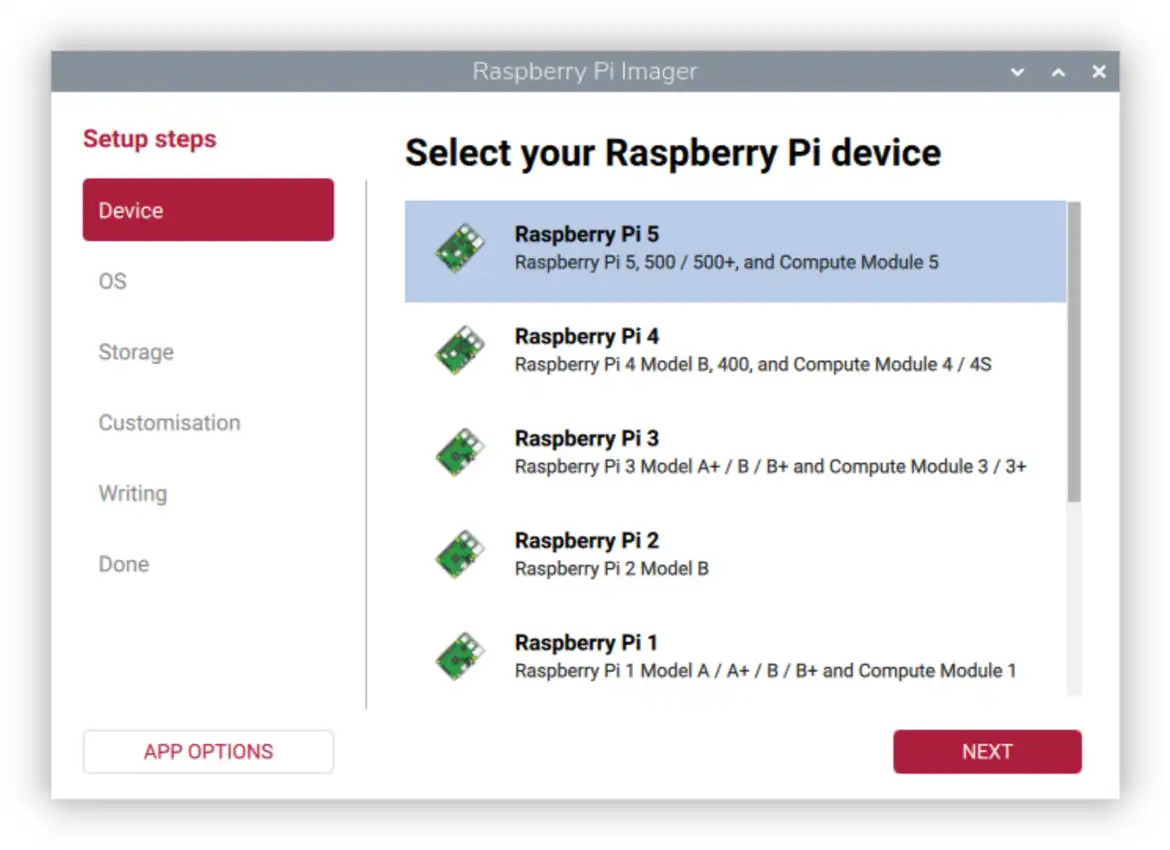
\includegraphics[width=\textwidth]{imager}
        \end{column}
        \begin{column}{.55\textwidth}
            Interface simple pour installer un OS

            \bigskip
            Pré-installé sur Raspberry Pi OS

            \bigskip
            Disponible pour toutes plateformes:

            \url{www.raspberrypi.com/software/}

        \end{column}
    \end{columns}
\end{frame}

\begin{frame}{Installation de DietPi}
    \begin{enumerate}
        \item Lancer Raspberry Pi Imager
        \item Sélectionner la carte Raspberry Pi 3
        \item Choisir "DietPi" dans la liste "Other general-purpose OS"
        \item Sélectionner la carte SD à écrire
        \item Redémarrer la Raspberry avec la carte SD remplacée
    \end{enumerate}

    \bigskip
    \bigskip
    \alert{Tip:} quand on installe un OS officiel Raspberry, on peut
    pré-configurer le système
\end{frame}

\begin{frame}{DietPi}{Un système d'exploitation au régime}
    \begin{columns}
        \begin{column}{.4\textwidth}
            \centering
            
\includegraphics[width=.8\textwidth]{dietpi}
        \end{column}
        \begin{column}{.6\textwidth}
            Basé sur Debian (comme Raspberry Pi OS)

            \alert{\(\rightarrow\) \cmd{apt}, \cmd{systemctl} disponibles}

            \bigskip
            Minimise:
            \begin{itemize}
                \item RAM
                \item CPU
                \item Stockage
                \item Packages pré-installés
            \end{itemize}

            \bigskip
            \url{dietpi.com}
        \end{column}
    \end{columns}
\end{frame}

\begin{frame}{Configuration initiale}

    Étapes principales:
    \begin{enumerate}
        \item Connexion en tant que \textit{root} (mot de passe par défaut
              donné)
        \item Configuration des utilisateurs par défaut (\textit{root} et
              \textit{dietpi})
        \item Création d'un mot de passe par défaut (attention sécurité: stocké
              en clair)
        \item \texttt{DietPi-Software} se lance automatiquement
              \begin{itemize}
                  \item accès à la configuration
                  \item installation facilitée de logiciels pré-configurés
                        (sur base de \cmd{apt})
              \end{itemize}
        \item Configurer le système et installer les logiciels voulus (cf.
              suite)
    \end{enumerate}
\end{frame}

\begin{frame}{Configuration du système}
    Dans \texttt{DietPi-Config}, régler:

    \begin{itemize}
        \item \textbf{Audio options}: sélectionner la carte son \texttt{rpi}
        \item \textbf{Display options}: activer les codecs Raspberry Pi
              (décodeur matériel performant)
        \item \textbf{Security options}: choisir un nom d'hôte
        \item \textbf{Network options}: configurer le Wi-Fi
    \end{itemize}

    \bigskip
    Dans \texttt{Browse Software}, installer:
    \begin{itemize}
        \item DietPi-Dashboard (interface web de contrôle du système)
        \item Avahi (résolution de nom d'hôte local)
    \end{itemize}

    \bigskip
    \alert{Tip:} utiliser \texttt{espace} pour sélectionner, \texttt{Enter} pour
    valider, \texttt{Esc} pour revenir en arrière
\end{frame}

\begin{frame}{La sélection de logiciels pré-configurés}
    DietPi offre une installation facilitée pour certains logiciels populaires

    \begin{itemize}
        \item \textbf{Desktops}: interfaces graphiques (LXDE)
        \item \textbf{Media Systems}: multimédia (Kodi, Jellyfin)
        \item \textbf{Gaming \& Emulation}: jeux vidéo
        \item \textbf{System Stats \& Management}: outils système
              (DietPi-Dashboard)
        \item \textbf{DNS Servers}: outils DNS (Pi-hole)
        \item \textbf{File Servers}: serveurs de fichiers (Samba)
        \item \textbf{VPN Servers}: serveurs VPN (Tailscale, similaire à
              Netbird)
        \item \textbf{Home Automation}: domotique (Home Assistant)
        \item \textbf{Development \& Programming}: outils de développement (Git,
              Python)
    \end{itemize}
\end{frame}

\begin{frame}{Les outils admin DietPi}{DietPi-Launcher et DietPi-Dashboard}
    \cmd{dietpi-launcher}: lister tous les outils offerts par DietPi

    \begin{itemize}
        \item \texttt{DietPi-Services}: basé sur \cmd{systemctl}, pour lister et
              contrôler les services
        \item \texttt{DietPi-CPUinfo}: afficher les informations sur le CPU
    \end{itemize}

    \bigskip
    \bigskip
    \begin{columns}
        \begin{column}{.55\textwidth}
            \texttt{DietPi-Dashboard}
            \begin{itemize}
                \item Interface web de gestion système
                \item Accès via \texttt{https://adresse\textunderscore IP:5252}
            \end{itemize}
        \end{column}
        \begin{column}{.45\textwidth}
            \centering
            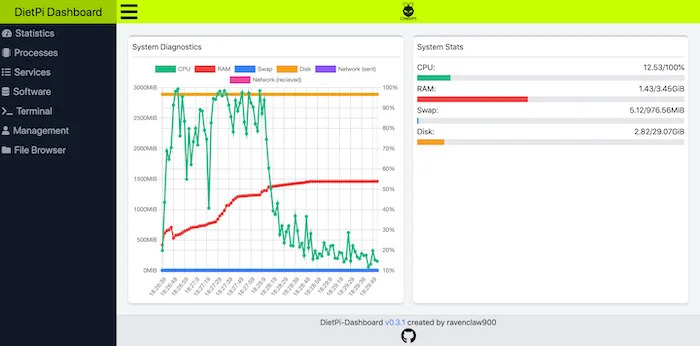
\includegraphics[width=\textwidth]{dashboard}
        \end{column}
    \end{columns}
\end{frame}

\begin{frame}{Fin de l'atelier}
    Récapitulatif des séances:
    \begin{enumerate}
        \item Introduction à Raspberry Pi
        \item Exploration du terminal Linux
        \item Programmation Python, GPIO et capteurs
        \item Utilisation de la caméra et de l'écran tactile
        \item Découverte de la domotique (Home Assistant)
        \item Création d'un serveur multimédia (Kodi, Jellyfin)
        \item Bases en réseau et VPN (Netbird)
        \item Bonus et projets libres
    \end{enumerate}

    \bigskip
    \alert{Ce n'est qu'un début!}

\end{frame}

\begin{frame}{Proposition bonus: streaming de jeux vidéo}{Sunshine \& Moonlight}

    Objectif: bénéficier de la puissance d'un PC gaming, même à distance

    \bigskip

    Sunshine est un serveur de streaming, optimisé pour le jeu vidéo

    \(\rightarrow\) installé sur une machine puissante qui fait tourner les jeux

    \medskip
    \url{app.lizardbyte.dev/Sunshine}

    \bigskip
    Moonlight est un client permettant de communiquer avec un serveur Sunshine

    \(\rightarrow\) installé sur le Raspberry Pi, connecté à un écran et à une
    manette
    \medskip

    \url{moonlight-stream.org}

\end{frame}

\begin{frame}{Conseils pour le projet Moonlight}
    Pour l'installation de Moonlight sur DietPi:
    \begin{enumerate}
        \item Utiliser \cmd{dietpi-software}
        \item Sélectionner la version GUI
        \item Utiliser \cmd{moonlight-qt} pour lancer le client
    \end{enumerate}

    \bigskip
    Pour le serveur Sunshine: suivre les instructions officielles pour votre
    machine

    \bigskip
    Étapes additionnelles:
    \begin{itemize}
        \item Être connecté au même réseau local que le serveur Sunshine
        \item Configurer le driver \textit{FKMS} dans \texttt{DietPi-Config}
              (display - resolution)
    \end{itemize}

\end{frame}

\end{document}
